\chapter{Results}


\subsection{The Simulation Environment} Testing in a simulation environment has been done using the URDF Gym Environment~\cite{spahn_urdfenvironment_2022}, a 100\% python environment build upon the PyBullet library \cite{coumans_pybullet_2016}. The code created during the thesis can be found on \href{https://gitlab.tudelft.nl/airlab-delft/msc_projects/msc_gijs_groote}{GitLab} and \href{https://github.com/GijsGroote/semantic-thinking-robot}{GitHub}. Experiments ran on standart TU Delft laptop: HP ZBook Studio x360 G5, running OS: Ubuntu 22.04.1 LTS x86\_64, CPU: Intel i7-8750H (12) @ 4.100GHz, GPU: NVIDIA Quadro P1000 Mobile.\bs
The simulation environment provides many different robot, 2 simple robots are selected to perform tests, they are displayed in \cref{fig:example_robots}, various obstacles are displayed in \cref{fig:example_obstacles}.

\begin{figure}[H]
    \centering
    \begin{subfigure}{.5\textwidth}
    \centering
    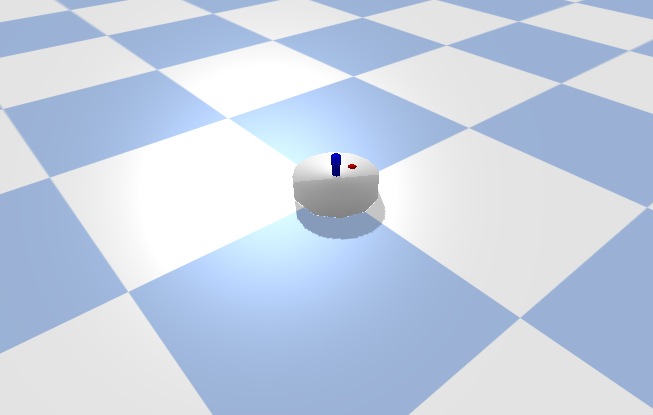
\includegraphics[width=0.8\textwidth]{figures/point_robot.png}
    \caption{The holonomic point robot\\the 2 inputs drive the robot in $x$ and in $y$ direction}
    \label{subfig:example_point_robot_todo_rename_this}
    \end{subfigure}%
    \begin{subfigure}{.5\textwidth}
    \centering
    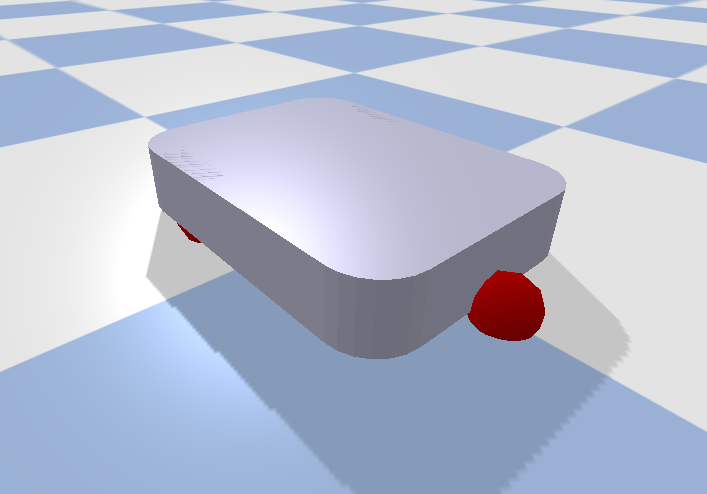
\includegraphics[width=0.8\textwidth]{figures/boxer_robot.png}
    \caption{The nonholonomic boxer robot\\the first input drives the robot forward/backward\\the second rotates the robot}
    \label{subfig:example_boxer_robot_todo_rename_this}
    \end{subfigure}%
    \caption{Robots used for testing, for either robot an velocity and a accelaration input exists, in total 4 different robots are used}
    \label{fig:example_robots_change_ref_please}

\end{figure}
\todo[inline]{renaem labels in thingy above}
\todo[inline]{zoom in a bit on these 2 cute robots}

\begin{figure}[H]
    \centering
    \begin{subfigure}{.5\textwidth}
    \centering
    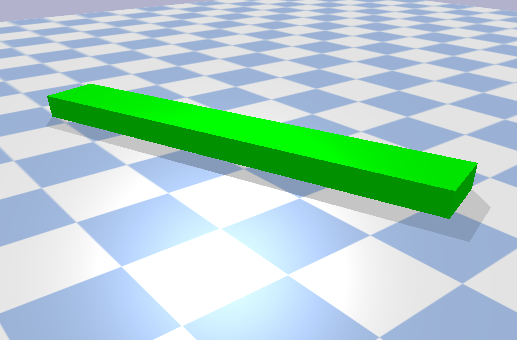
\includegraphics[width=0.8\textwidth]{figures/box_obstacle.png}
    \caption{A box obstacle}
    \end{subfigure}%
    \begin{subfigure}{.5\textwidth}
    \centering
    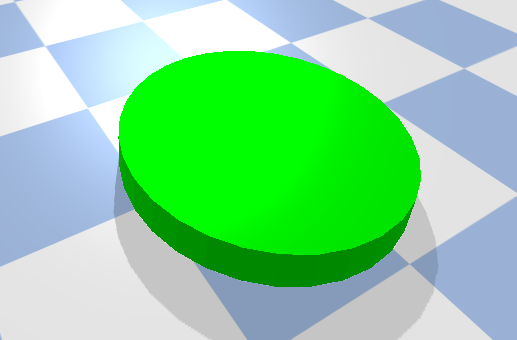
\includegraphics[width=0.8\textwidth]{figures/cylinder_obstacle.png}
    \caption{A cylinder obstacle}
    \end{subfigure}%
    \caption{Various obstacles in the robot environment}
    \label{fig:example_obstacles_change_this_label}
\end{figure}



The results will be made in a while, wait for a moment while we try to make sense of the almost existing results



\section{Metrics}

A clear distinction between a transition, or an hypothesis is now made. A transition is a single action. An hypothesis is an sequence of actions/transitions.\\


\todo[inline]{why would any metric be usefull, explain why a metric is required.}

\textbf{Metric for a transition}
\newline
Prediction Error\\
Tracing Error\\
Failing/succeeding of this  transition\\
(optional) model accuracy (if you can get the model from the pybullet simulation
number of collisions
repositioning around an object when pushing
number of replanning of motion planning\\
final position and displacement error\\

\todo[inline]{Split metrics in internal and external/comparable}

\textbf{Metric for hypothesis}
\newline
Number of replanning an hypothesis\\
number of Successes/number of failed transitions in the hypothesis\\
overall planning time\\
overall runtime\\
completion time = runtime + planning time\\
fail/success of the task\\
number of hypothesis / number of target positions\\

\textbf{Metric for executing a task}
completion / uncompleted subtasks


\textbf{System identification}
\newline
estimation of object mass\\
Comparison of bode diagram\\
poles and zeros of the true and estimated model.\\


\newpage
\section{Benchmark Tests}
\section{Comparison with related papers}
The papers to compare with:\newline

\citefield{sabbaghnovin_model_2021}{title}\\

\cite{sabbaghnovin_model_2021}, 
\todo[inline]{See the paper for tests to reproduce with my hgraph}


\citefield{novin_dynamic_2018}{title}\\
\cite{novin_dynamic_2018}
The following \cite{novin_dynamic_2018} citation is here because it is a refered to from \cite{sabbaghnovin_model_2021} many times
\section{Randomisation}
\section{Knowledge Graph On/Off}
